%% Artyom Voronin
%%  __     _ _                   
%% / _| __| (_)  _ __  _ __ ___  
%%| |_ / _` | | | '_ \| '_ ` _ \ 
%%|  _| (_| | | | |_) | | | | | |
%%|_|  \__,_|_| | .__/|_| |_| |_|
%%              |_|              
%% Brno, 2021
\documentclass[class=article, crop=false]{standalone}
\usepackage[subpreambles=true]{standalone}
\usepackage{subcaption}

\usepackage{sectsty}
\usepackage{graphicx}
\graphicspath{{img/}{../img/}{../../img/}}
\usepackage{listings}
\lstset{language=Matlab}
\usepackage{hyperref}
\usepackage{amsmath}
\usepackage{import}
\usepackage{subfiles}
\usepackage[utf8]{inputenc}
\usepackage[english]{babel}

%\usepackage[square, numbers]{natbib}
%\bibliographystyle{unsrtnat}
%\usepackage[nottoc]{tocbibind}

%\usepackage{biblatex}
%\addbibresource{./citations.bib} %usage \cite{test}
% Margins
% 
\topmargin=-0.45in
\evensidemargin=0in
\oddsidemargin=0in
\textwidth=6.5in
\textheight=9.0in
\headsep=0.25in

%\title{PM and FDI comparison}
%\author{Artyom Voronin} 
%\date{}

\begin{document}

\section{PM and FDI comparison}

The relative arrangement PM and FDI methods representing in following
figure \ref{fig:fdi_pm}
\begin{figure}[h!]
    \centering
    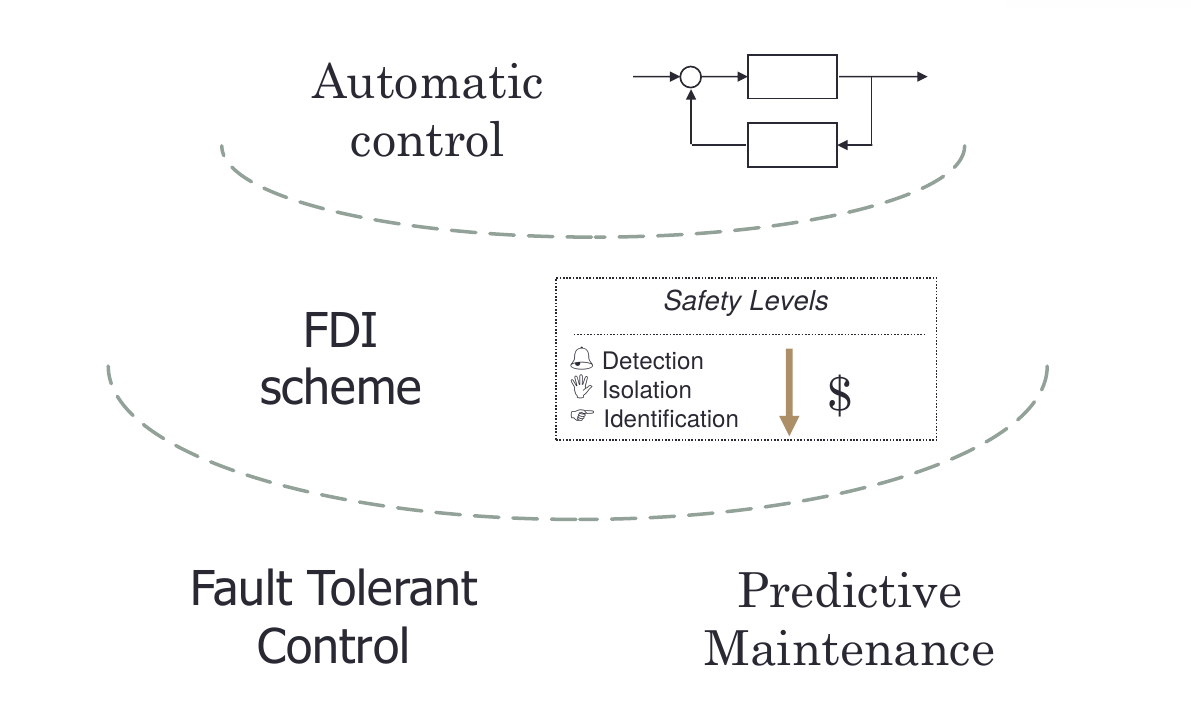
\includegraphics[scale=0.3]{FDI_PM.png}
    \caption{PM and FDI }
    \label{fig:fdi_pm}
\end{figure}

\subsection{Fault detection and isolation}


%\textbf{Fault \footnotemark detection and isolation} is subfield of control
%engineering, identifying when fault  has occurred, and pinpointing the type
%of fault and its location.

\footnotetext{\textbf{Fault} - not acceptable deviation of at least one characteristic or
parameter of the system from the standard condition.}
 
\textbf{Fault diagnosis}:
\begin{itemize}
    \item{Fault detection: Detect malfunctions in real time, as soon and as
        surely as possible.}
    \item{Fault isolation: Find the root cause, by isolating the system
        components whose operation mode is not nominal.}
    \item{Fault identification: Estimation the size and type or nature of the
        fault.}
\end{itemize}

\textbf{There are two common approaches for fault detection
\ref{fig:fault_detection}}:
\begin{itemize}
\item{Model-based FDI (compare data with healthy-model)}
\item{Signal processing based FDI (using math methods to extract information
    about the fault from data)}
\end{itemize}

\begin{figure}[h]
    \centering

\begin{subfigure}{0.5\textwidth}
    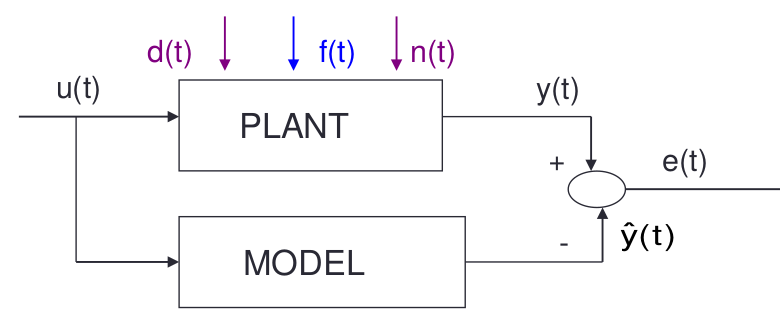
\includegraphics[width=0.9\linewidth]{model_based.png}
    \caption{Model-based fault detection}
    \label{fig:model_based}
\end{subfigure}%
\begin{subfigure}{0.5\textwidth}
    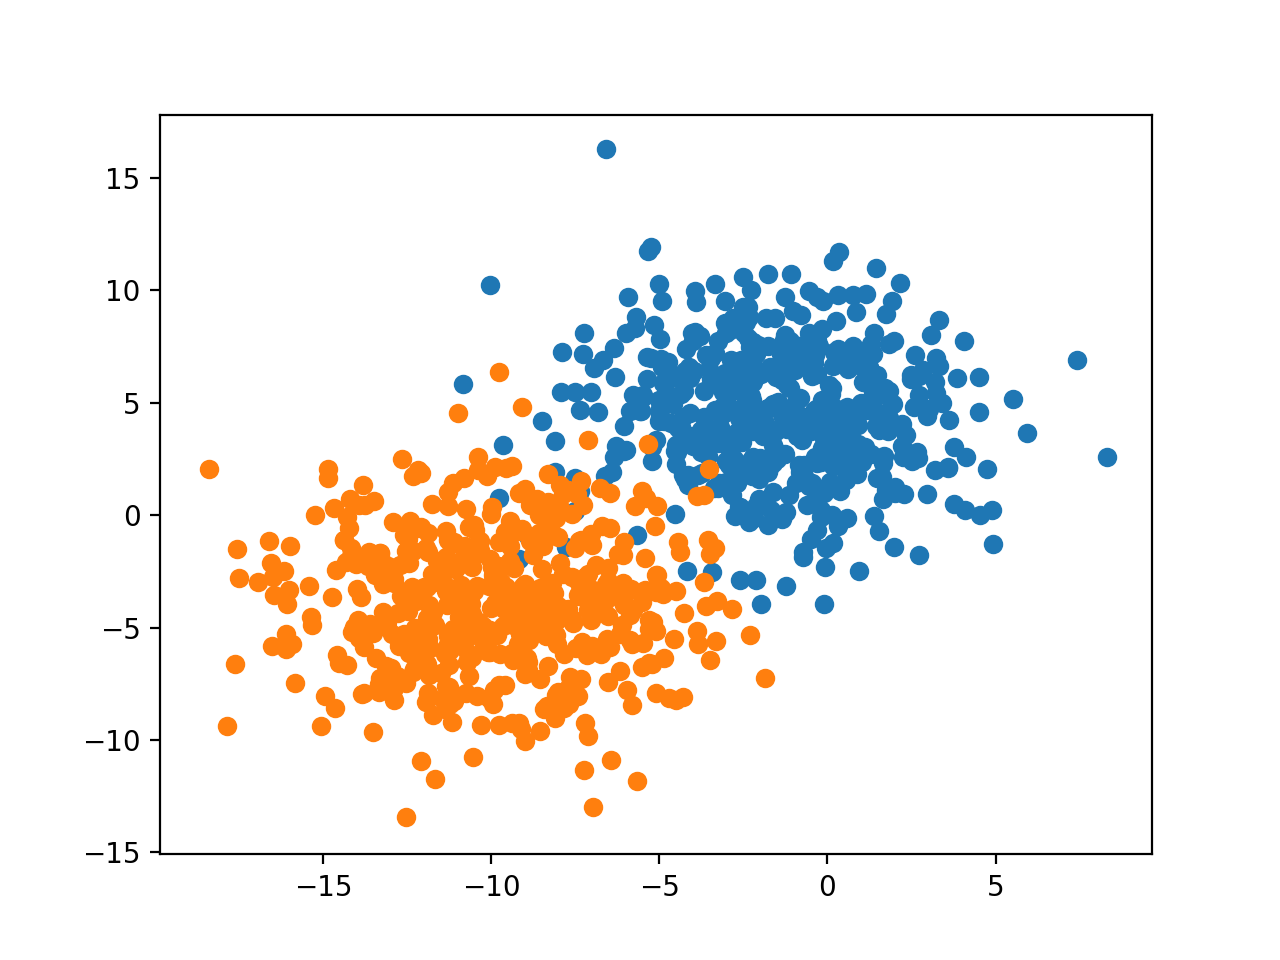
\includegraphics[width=0.9\linewidth]{signal_based.png}
    \caption{Signal-based fault detection}
    \label{fig:signal_based}
\end{subfigure}

\caption{Fault detection common approaches}
\label{fig:fault_detection}

\end{figure}

The result of FDI is the detection and identification of faults that occur
during the operation of the device. Subsequently data is processed using
Fault Tolerance and Predictive maintenance methods.


\subsection{Fault Tolerance}
\textbf{Fault Tolerance}: Provide the system with the hardware architecture and
  software mechanisms which will allow, if possible to achieve a given
  objective not only in normal operation, but also in given fault
  situations.


\subsubsection{Predictive maintenance}
\textbf{Predictive maintenance} is cost-effective maintenance strategy that
predicts time to failure and warns of an anticipated location where this
could occur.
Predict where, when and what is the reason of failure (identify primary
factors).

The are two main goals of Predictive maintenance, RUL (remaining useful
life) and identification where the future failure can appear, or what is
the reason of decreasing RUL.



\textbf{Types of Maintenance}:
\begin{itemize}
    \item{Reactive (fails than fix)}
    \item{Preventative (schedules)}
    \item{Condition-based (based on assess of system)}
    \item{Predictive (based on model that predict failure)}
\end{itemize}

\textbf{Predictive maintenance development sequence}:
\begin{enumerate}
    \item{Collect data (using sensors, math model)}
    \item{Process data (clean up data)}
    \item{Identify condition indicators CI}
        \begin{itemize}
            \item{Signal-based CI}
            \item{Model-based CI}
        \end{itemize}
    \item{Fit model (ML techniques)}
    \item{Deploy monitoring and integrate}
    \item{Dashboard (UI)}
\end{enumerate}

As a result of PM is RUL representing of number cycles, days, or some time
period before fault occurred. And probability where this fault can appear.

\subsection{Methods}
There are couples of signal processing and analysing methods that used in
both PM and FDI. For example:
\begin{itemize}
    \item Spectral Analysis
    \item Wavelet Analysis
    \item Wavelet transform
    \item FFT
    \item Short Term Fourier Transform
    \item Gabor Expansion
    \item Wigner-Ville distribution
    \item Correlation
    \item High resolution spectral analysis
    \item Waveform Analysis
    \item Time-Frequency Analysis
    \item PCA
    \item Machine Learning techniques:
        \begin{itemize}
            \item kNN
            \item ANN
        \end{itemize}
\end{itemize}

%\medskip
%\printbibliography

\end{document}

